%preamble
\documentclass[12pt,a4paper]{article}

%inputs for firstpage
\def \CourseName {گزارش فاز دوم}
\def \Instructor {دکتر مسلم حبیبی}
\def \Semester {نیم‌سال دوم\\سال تحصیلی 99-00}


%packages
\usepackage[]{algorithm2e}
\usepackage{cite}
\usepackage{calc}
\usepackage{fancyhdr}
\usepackage{lipsum}
\usepackage{color}
\usepackage{ragged2e}
\usepackage[inline]{enumitem}
\usepackage[dvipsnames]{xcolor}
\usepackage{graphicx}
\usepackage{wrapfig}
\usepackage{float}
\usepackage[skip=12pt,indent=2em]{parskip}
\usepackage{setspace}
\usepackage{textcomp}
\usepackage{etoolbox}
\usepackage{xpatch}
\usepackage{tabu}
\usepackage{hyperref}


%for persian fonts
\usepackage{xepersian}
\defpersianfont\bnazanin{BNazanin}
\settextfont{BNazanin}

\title{
	\center
	
\includegraphics[width=5cm, height=5cm]{images/shariflogo.jpg} \\
	دانشکده مهندسی صنایع \\
	دانشگاه صنعتی شریف \\
	\CourseName
}
\author{
	\\
	\\
	\textbf{استاد درس:}
	\\
	\Instructor \\[35pt]
	\\
	\textbf{نام اعضای گروه:}
	\\مهدی محسنی 
	\\محراب کشاورز گیلده 
	\\احسان چشمی
	\\[45pt]
}
\date{{\small\Semester}}


%body
\begin{document}

\maketitle
\pagebreak
\tableofcontents
\pagebreak
\listoffigures
\pagebreak
\normalsize	

\section{نمودار موردکاربرد} \label{section.useCase}
	\begin{figure}[h!]
		\begin{center}
			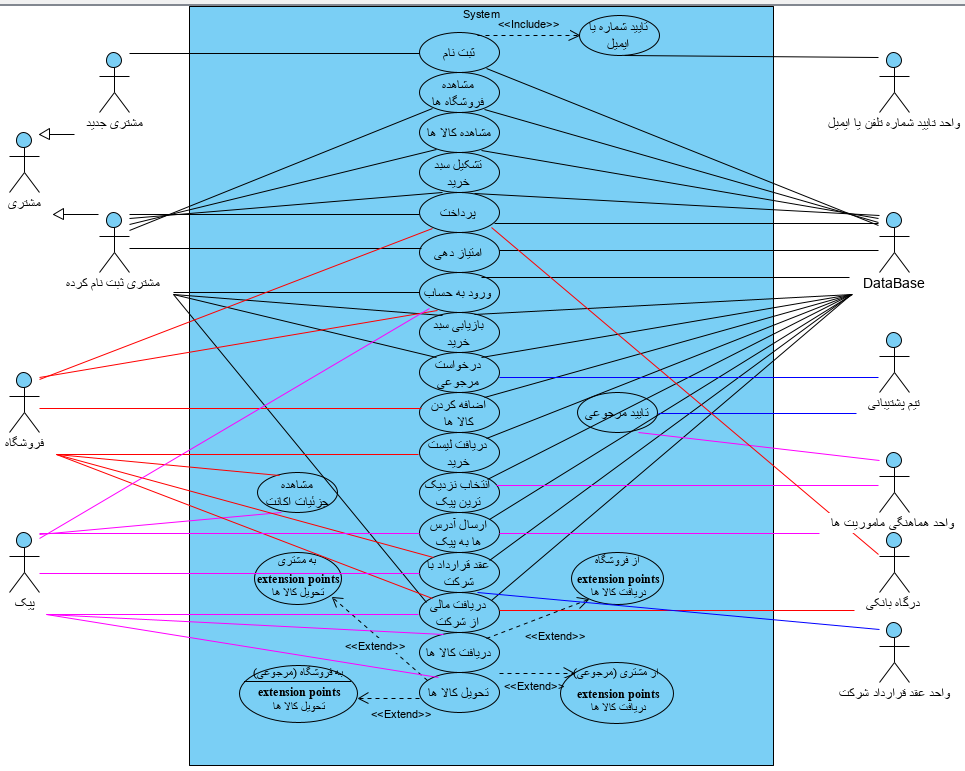
\includegraphics[width=12cm]{images/Use Case.png}
			
		\end{center}
		\caption{نمودار مورد کاربرد}
	\end{figure}
 

\textbf{توضیحات :} 
	\begin{enumerate}
		\item 
		آکتورهای مشتری جدید و مشتری ثبت نام شده را با یک رابطه ارث بری به آکتور والد مشتری متصل می کنیم.
		\item
		فرض بر این بوده که مشتری تنها بعد ثبت نام میتواند لیست فروشگاه ها و کالاها را ببیند.
		\item
		منظور از یوزکیس بازیابی سبد خرید، بعد از پرداخت ناموفق است.
		\item
		فرض بر این بوده تمام دیتاها از جمله موجودی کالاها، جزییات حساب ها، تاریخچه پرداخت ها و غیره در دیتابیس شرکت ذخیره می شود.
		\item
		منظور از یوزکیس دریافت مالی از شرکت دریافت مبلغ فروش توسط فروشگاه،درآمد پیک از تحویل کالا و مبلغ بازگشتی به مشتری در صورت مرجوع کردن کالا می باشد.
		\item
		آکتور واحد هماهنگی ماموریت ها وظیفه دریافت اطلاعات پیک ها از دیتابیس شرکت، پیدا کردن نزدیکترین پیکی که ماموریت را بپذیرد، و سپردن ماموریت دریافت و تحویل کالا به پیک را دارد.
	\end{enumerate}
\pagebreak
\section{نمودارهای فعالیت} \label{section.activity}
	\subsection{فرایند ثبت نام} \label{section.activity.register}
		\begin{figure}[h!]
			\begin{center}
				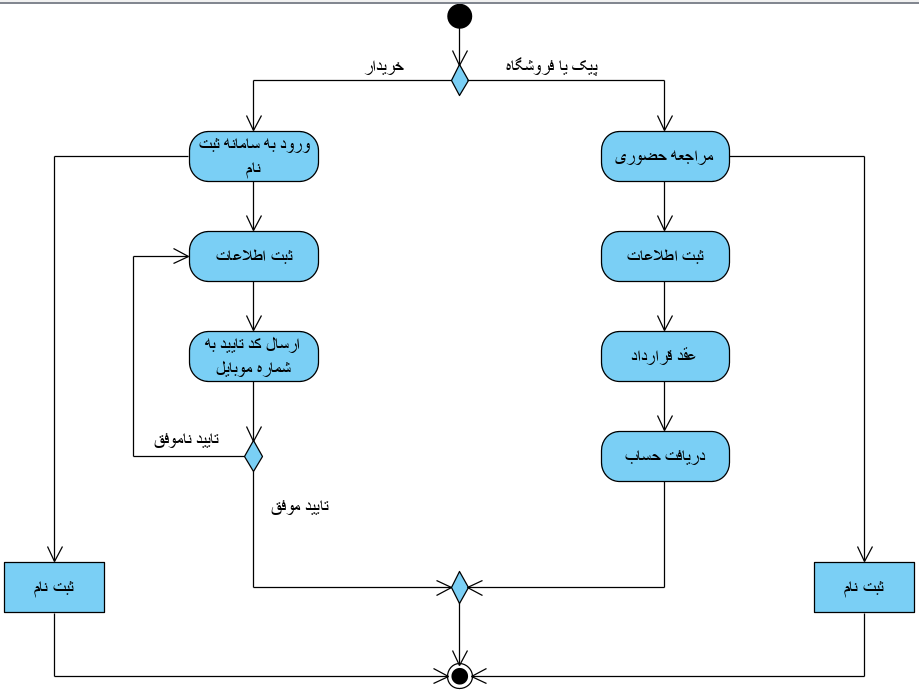
\includegraphics[width=14cm]{images/Register Activity Diagram.png}
			\end{center}
			\caption{نمودار فعالیت ثبت نام}
		\end{figure}
	
	\textbf{توضیحات :} 
	
	
	خریدار برای ثبت نام وارد سامانه می شود، اطلاعات خود را وارد میکند و کد تایید به شماره یا ایمیل او ارسال می شود. در صورت عدم تایید شماره یا ایمیل دوباره به مرحله ثبت اطلاعات بازمی گردد و در صورت تایید ثبت نام تایید می گردد.	پیک یا صاحب فروشگاه برای ثبت نام به صورت حضوری مراجعه می کنند، اطلاعات خود را به متصدی ثبت نام می دهند و قرار داد امضا می کنند سپس حساب کاربری خود در سامانه را دریافت می کنند.
\pagebreak	
	\subsection{فرایند خرید} \label{section.activity.buy}
	
	
	
	\subsection{فرایند مرجوعی} \label{section.activity.return}
		\begin{figure}[h!]
			\begin{center}
				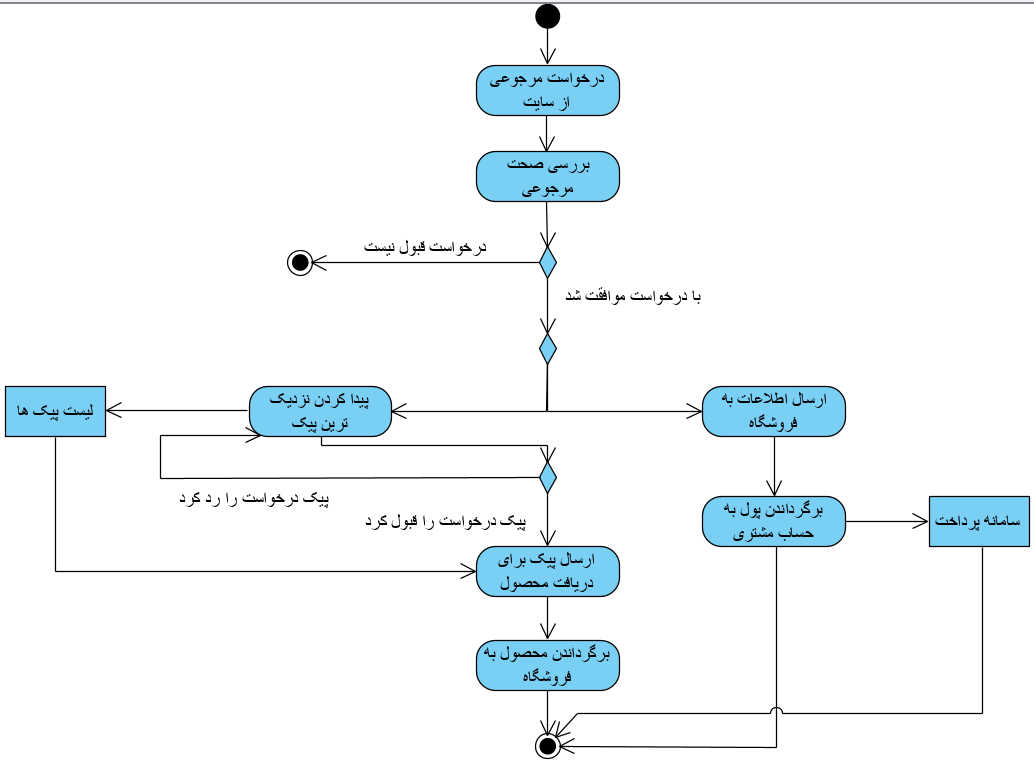
\includegraphics[width=14cm]{images/Return Activity Diagram.png}
			\end{center}
			\caption{نمودار فعالیت مرجوعی}
		\end{figure}
		
	\textbf{توضیحات :} 
	
	
	پس از بررسی صحت درخواست مرجوعی مشتری در صورتی که درخواست غیر منطقی باشد و قابل قبول با قوانین تایید شده در هنگام خرید نباشد درخواست رد می شود در غیر این صورت درخواست قبول می شود و دو اتفاق می افتد:
	\begin{enumerate}
		\item
		اطلاعات مرجوعی به فروشگاه داده می شود تا پول را پس دهد.
		\item
		نزدیک ترین پیک پیدا می شود تا محصول را از مشتری دریافت کند و به فروشگاه برگرداند.
	\end{enumerate}
	\textbf{نکته: }دو قسمت \underline{لیست پیک ها }و \underline{سامانه پرداخت} آبجکت هستند و اتصال به آن ها باید با خط چین باشد اما ویژوال پارادایم آن ها را خط گذاشته است.
	
\pagebreak

\section{نمودارهای توالی} \label{section.sequence}

	
	\subsection{فرایند ثبت نام} \label{section.sequence.register}
	
	
	\subsection{فرایند خرید} \label{section.sequence.buy}
	
	
	\subsection{فرایند مرجوعی} \label{section.sequence.return}
	
	

\pagebreak

\section{گزارش نحوه انجام پروژه} \label{section.report}
	
	\subsection{جلسه \lr{post mortem}} \label{section.report.postMortem}
	
	\pagebreak
	
	\subsection{\lr{Task board and Burndown Chart}} \label{section.report.taskBoard}
			\begin{figure}[h!]
			\begin{center}
				\includegraphics[width=9cm]{images/screenshot_1.png}	
			\end{center}
			\caption{ابتدای اسپرینت-بخش اول}
		\end{figure}
		
		\begin{figure}[h!]
			\begin{center}
				\includegraphics[width=9cm]{images/screenshot_2.png}
			\end{center}
			\caption{ابتدای اسپرینت-بخش دوم}
		\end{figure}
			\begin{figure}[h!]
			\begin{center}
				\includegraphics[width=9cm]{images/screenshot_3.png}	
			\end{center}
			\caption{ابتدای اسپرینت-بخش سوم}
		\end{figure}
		
		\begin{figure}[h!]
			\begin{center}
				\includegraphics[width=9cm]{images/screenshot_4.png}
			\end{center}
			\caption{انتهای اسپرینت-بخش اول}
		\end{figure}
			\begin{figure}[h!]
			\begin{center}
				\includegraphics[width=9cm]{images/screenshot_5.png}	
			\end{center}
			\caption{انتهای اسپرینت-بخش دوم}
		\end{figure}
		
		\begin{figure}[h!]
			\begin{center}
				\includegraphics[width=9cm]{images/screenshot_6.png}
			\end{center}
			\caption{انتهای اسپرینت-بخش سوم}
		\end{figure}
	
	\pagebreak
	
	
	\begin{figure}[h!]
		\begin{center}
			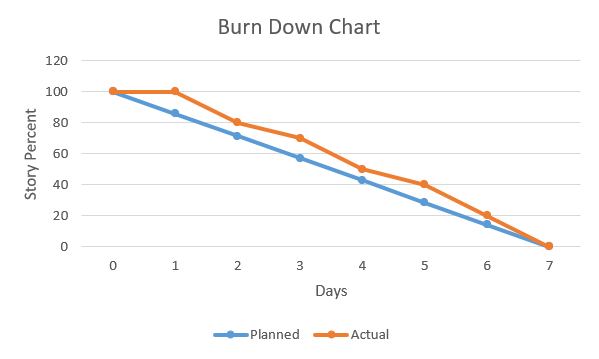
\includegraphics[width=14cm]{images/Burn Down Chart.png}
			
		\end{center}
		\caption{\lr{Burn Down Chart}}
	\end{figure}
	
	
	

\end{document}